\documentclass[aspectratio=169,11pt]{beamer}

\usepackage{amsmath,amssymb}
\usepackage{graphicx}
\usepackage{booktabs}
\usepackage{xcolor}

\graphicspath{{figures/}}
\newcommand{\Lc}{\mathcal{L}}
\usetheme{Madrid}
\usecolortheme{seahorse}
\setbeamertemplate{navigation symbols}{}
\setbeamertemplate{caption}[numbered]
\setbeamerfont{caption}{size=\scriptsize}

\title[MLP from Scratch]{Studying Loss Functions and the Training Criterion}
\subtitle{Implementation in NumPy and empirical study on MNIST}
\author[Martirosov]{Daniel James Martirosov\\ \small ID 24948933 \quad 2026}
\institute[A2]{Advanced Data Analytics Algorithms, Machine Learning\\ Assessment Task 2}
\date{}

\begin{document}

\begin{frame}
  \titlepage
  \begin{center}
  \footnotesize
  Notebook: \url{https://github.com/MathgeniusTB2/a2-mlp-from-scratch/blob/main/a2_mlp_numpy.ipynb}
  \end{center}
\end{frame}

\begin{frame}{Task and inputs/outputs (head first)}
  \textbf{Task:} classify a hand-written digit into one of ten classes.
  \vspace{0.4em}
  \begin{columns}[T]
    \begin{column}{0.5\textwidth}
      \textbf{Training}
      \begin{itemize}
        \item Input: $28\times28$ image of integers in $[0,255]$, normalised to $[0,1]$, flattened to $\mathbb{R}^{784}$.
        \item Target: one-hot vector in $\{0,1\}^{10}$.
      \end{itemize}
    \end{column}
    \begin{column}{0.5\textwidth}
      \textbf{Deployment}
      \begin{itemize}
        \item Input: one image, same deterministic preprocessing.
        \item Output: $p\in[0,1]^{10}$, $\sum_k p_k=1$; decision $\arg\max_k p_k$.
      \end{itemize}
    \end{column}
  \end{columns}
  \vspace{0.5em}
  \textbf{Research question:} how does the choice of training criterion change what the network
  learns, and when does minimising the loss fail to serve the task objective?
\end{frame}

\begin{frame}{The five criteria}
  Same MLP $784\text{-}128\text{-}128\text{-}10$ (tanh, 118\,282 params); only the loss changes.
  \vspace{0.4em}
  \begin{columns}[T]
    \begin{column}{0.5\textwidth}
      \small
      \begin{itemize}
        \item \textbf{Cross-entropy}: $-\frac1n\sum y\log\hat p$ (proper, reference).
        \item \textbf{Squared error}: $\frac1n\sum\tfrac12\lVert\hat p-y\rVert^2$.
        \item \textbf{Absolute error}: $\frac1n\sum\lVert\hat p-y\rVert_1$.
        \item \textbf{Label smoothing}: CE against $(1-\epsilon)y+\epsilon/K$.
        \item \textbf{Expected cost (mine)}: $\frac1n\sum\hat p_k(1-R_{y,k})$.
      \end{itemize}
    \end{column}
    \begin{column}{0.46\textwidth}
      \textbf{My reward matrix}\\
      \small rows = true digit, columns = guess; diagonal 10, visually similar digits get up to
      6 (e.g. $4{:}9=6$, $3{:}5=5$). The criterion is the expected cost of the decision, so a
      near miss is cheaper.
    \end{column}
  \end{columns}
\end{frame}

\begin{frame}{Gradients: theory to code}
  \begin{block}{Only $\delta^{(L)}=\partial\Lc/\partial z^{(L)}$ changes between criteria}
  \small
  \begin{tabular}{@{}ll@{}}
  \toprule
  Criterion & logit gradient \\
  \midrule
  cross-entropy & $\frac1n(\hat p-y)$ \\
  squared error & $\frac1n\hat p\odot\big((\hat p-y)-\sum_k(\hat p_k-y_k)\hat p_k\big)$ \\
  absolute error & $\frac1n\hat p\odot\big(\mathrm{sign}(\hat p-y)-\sum_k\mathrm{sign}(\hat p_k-y_k)\hat p_k\big)$ \\
  label smoothing & $\frac1n(\hat p-t)$ \\
  expected cost & $\frac1n\hat p\odot\big(c-\sum_k\hat p_k c_k\big)$, $c=1-R_y$ \\
  \bottomrule
  \end{tabular}
  \end{block}
  \small
  Weight gradient is shared: $\partial\Lc/\partial W^{(\ell)}=\delta^{(\ell)\top}a^{(\ell-1)}$.
  The softmax Jacobian gives the $\hat p_k(g_k-\sum_j\hat p_j g_j)$ form.
\end{frame}

\begin{frame}{Learning algorithm and protocol}
  \begin{columns}[T]
    \begin{column}{0.5\textwidth}
      \textbf{Mini-batch Adam}, $\eta=10^{-3}$, 30 epochs
      \[
      \theta \leftarrow \theta-\eta\,\frac{\hat m}{\sqrt{\hat v}+\epsilon}
      \]
      \begin{itemize}
        \item Bias-corrected moments, written from scratch.
        \item Same optimiser and rate for all five criteria.
      \end{itemize}
    \end{column}
    \begin{column}{0.5\textwidth}
      \textbf{Honest protocol}
      \begin{itemize}
        \item 5-fold cross-validation on the training set $\to$ compare criteria (folds are validation, \emph{not} test).
        \item Refit on all 60\,000, score \textbf{once} on t10k, over 3 seeds.
        \item Majority-class baseline: 11.4\%.
      \end{itemize}
    \end{column}
  \end{columns}
\end{frame}

\begin{frame}{Training over time}
  \begin{columns}[T]
    \begin{column}{0.78\textwidth}
      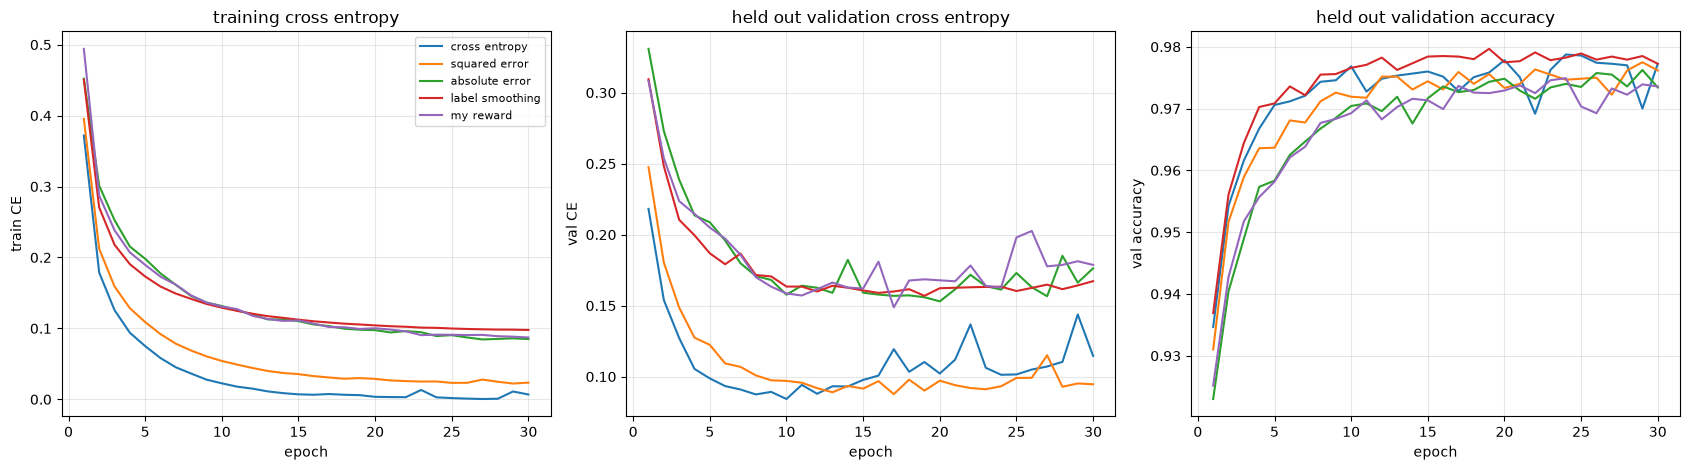
\includegraphics[width=\textwidth]{fig_learning_curves.png}
    \end{column}
    \begin{column}{0.2\textwidth}
      \begin{itemize}
        \item Train CE falls; held-out validation CE flattens.
        \item The gap is ordinary overfitting.
        \item Validation is a held-out fold --- never the train set, or the curve would only show fit.
      \end{itemize}
    \end{column}
  \end{columns}
\end{frame}

\begin{frame}{Results}
  \begin{columns}[T]
    \begin{column}{0.55\textwidth}
      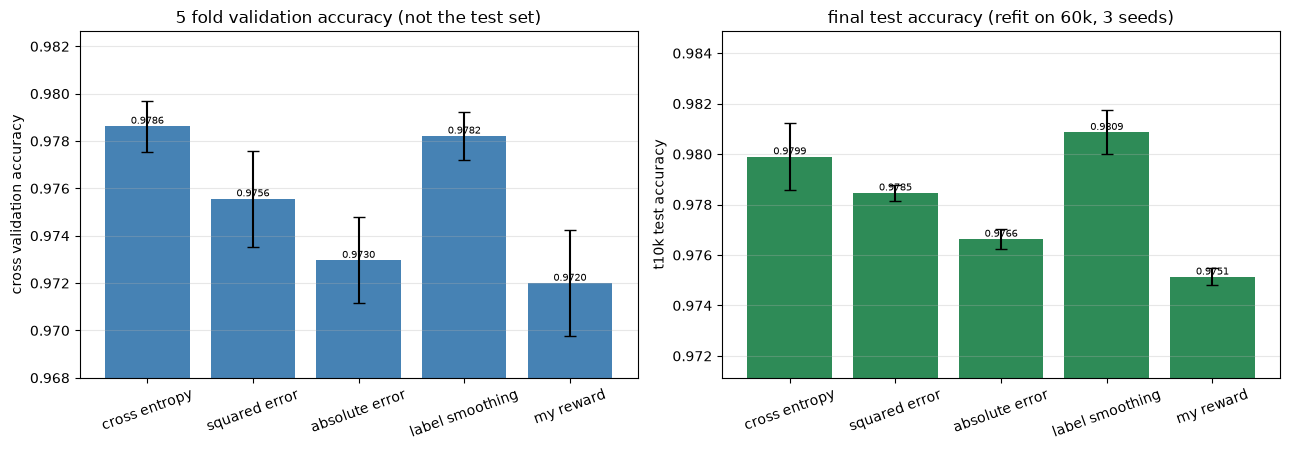
\includegraphics[width=\textwidth]{fig_criterion_comparison.png}
    \end{column}
    \begin{column}{0.43\textwidth}
      \scriptsize
      \begin{tabular}{@{}lrr@{}}
      \toprule
      Criterion & CV & Test acc. \\
      \midrule
      label smooth & 0.9782 & \textbf{0.9809} \\
      cross entropy & 0.9786 & 0.9799 \\
      squared error & 0.9756 & 0.9785 \\
      absolute error & 0.9730 & 0.9766 \\
      my reward & 0.9720 & 0.9751 \\
      \bottomrule
      \end{tabular}
      \vspace{0.4em}
      \begin{itemize}
        \item Accuracy spreads $0.9751$--$0.9809$; choice matters.
      \end{itemize}
    \end{column}
  \end{columns}
\end{frame}

\begin{frame}{Loss versus task objective}
  \begin{columns}[T]
    \begin{column}{0.5\textwidth}
      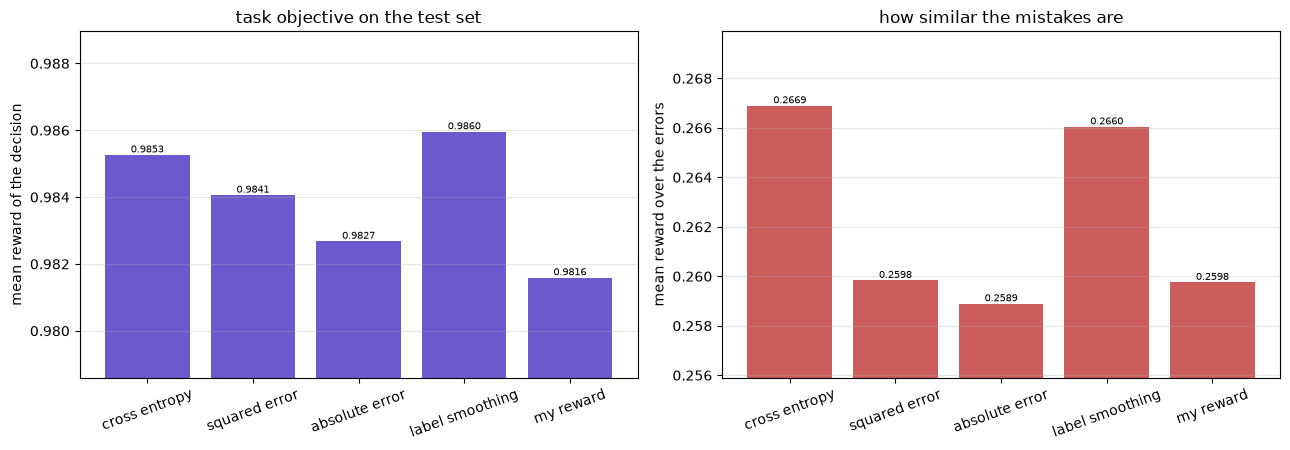
\includegraphics[width=\textwidth]{fig_task_objective.png}
    \end{column}
    \begin{column}{0.47\textwidth}
      \begin{itemize}
        \item \textbf{Lowest test CE: squared error (0.0826)} --- but not the most accurate.
        \item \textbf{Highest accuracy: label smoothing (0.9809)} --- but only third-lowest CE (0.1558).
        \item Loss scores the whole probability vector; accuracy scores only the arg max.
        \item Label smoothing vs cross-entropy is \emph{not} distinguishable (0.0010 apart, $\sim$1 SE).
        \item My expected-cost criterion is last on accuracy (0.9751).
      \end{itemize}
    \end{column}
  \end{columns}
\end{frame}

\begin{frame}{Calibration}
  \begin{columns}[T]
    \begin{column}{0.5\textwidth}
      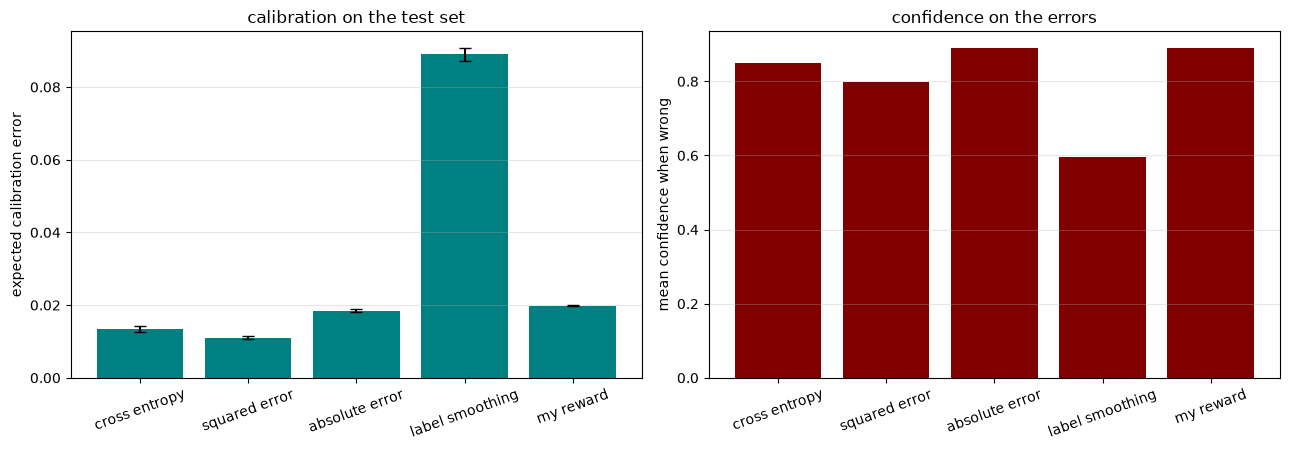
\includegraphics[width=\textwidth]{fig_calibration.png}
    \end{column}
    \begin{column}{0.47\textwidth}
      \begin{itemize}
        \item Measured ECE: squared error 0.011 (best), cross-entropy 0.014, \textbf{label smoothing 0.089 (worst)}.
        \item Label smoothing is the most accurate but the least calibrated (capped confidence, under-confident).
        \item Mean confidence on errors: 0.60 (label smoothing) vs 0.85 (cross-entropy).
      \end{itemize}
    \end{column}
  \end{columns}
\end{frame}

\begin{frame}{Why the linear criteria fail}
  \begin{columns}[T]
    \begin{column}{0.5\textwidth}
      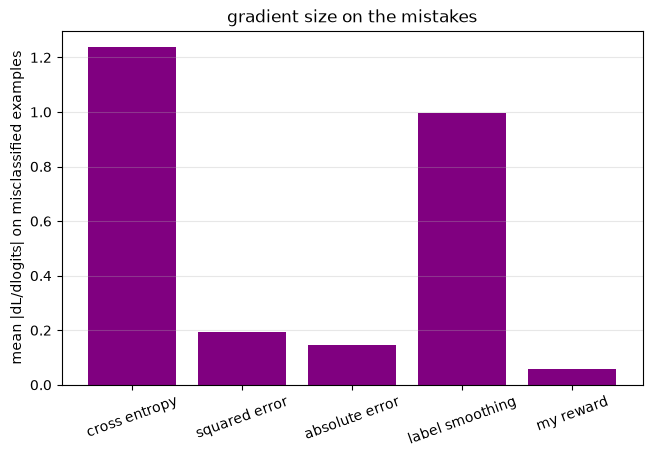
\includegraphics[width=\textwidth]{fig_gradient_norms.png}
    \end{column}
    \begin{column}{0.47\textwidth}
      \begin{itemize}
        \item For squared error, absolute error and expected cost, $\delta=\hat p\odot(g-\sum_j\hat p_j g_j)$: the gradient carries a factor $\hat p_k$ and \textbf{vanishes when confidently wrong}.
        \item Cross-entropy's $\delta=\hat p-y$ does not.
        \item Gradient norm on the mistakes: CE 1.24, label smoothing 1.00, squared 0.19, absolute 0.15, mine 0.06.
        \item Absolute error is hidden-linear: $\lVert\hat p-y\rVert_1=2(1-\hat p_y)$.
      \end{itemize}
    \end{column}
  \end{columns}
\end{frame}

\begin{frame}{Where the mistakes land}
  \begin{columns}[T]
    \begin{column}{0.72\textwidth}
      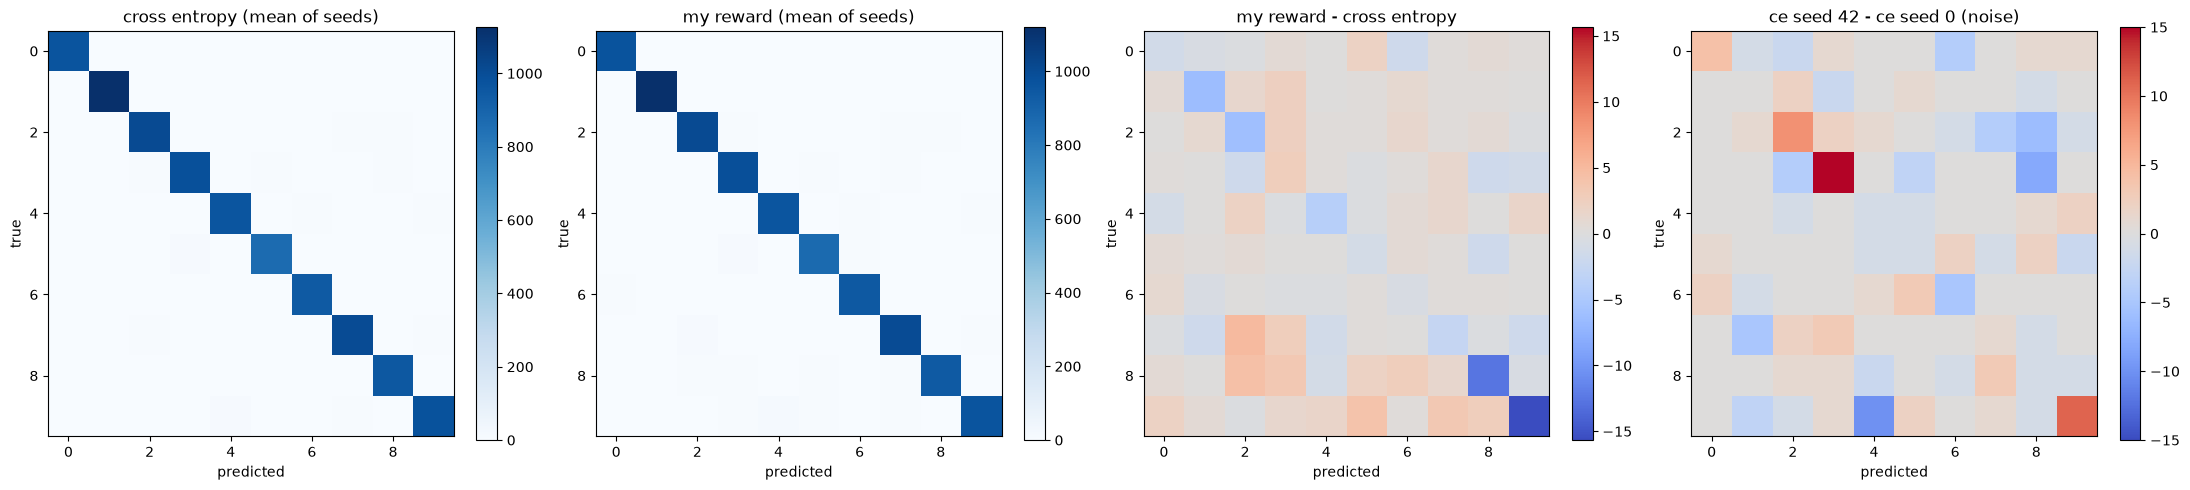
\includegraphics[width=\textwidth]{fig_confusion_matrices.png}
    \end{column}
    \begin{column}{0.26\textwidth}
      \begin{itemize}
        \item Cross-entropy vs my reward, their difference, and a seed-to-seed noise baseline.
        \item Largest cell change 15.7 vs noise 15.0: within run-to-run noise.
        \item The designed cost changed individual errors, not the aggregate; the $3/5/8$ and $4/9$ structure is the same.
      \end{itemize}
    \end{column}
  \end{columns}
\end{frame}

\begin{frame}{Limitations and summary}
  \textbf{Limitations}
  \begin{itemize}
    \item Single hand-designed reward matrix; a data-derived one could differ.
    \item No finite-difference gradient check; calibrated in-sample; no early stopping.
    \item Two tanh layers, 30 epochs, 3 seeds: large gaps solid, sub-0.1-point gaps are not.
  \end{itemize}
  \vspace{0.4em}
  \textbf{Summary}
  \begin{itemize}
    \item The criterion changes accuracy by ~0.6 points under identical training.
    \item Loss and objective disagree: lowest CE (squared error) is not the most accurate; label
          smoothing is the most accurate but the worst calibrated.
    \item The two improper, linear criteria finish last and second-last; their gradient norm on
          the mistakes is far smaller, consistent with the vanishing-gradient explanation.
  \end{itemize}
\end{frame}

\end{document}
